% ============================================================
% 5. RESULTS & ANALYSIS
% ============================================================
\section{Results \& Analysis}

\subsection{Main Effect: TPE Improves Emotional Variance Without Collapse}

Table~\ref{tab:main} shows the core result. On \textbf{qwen3-max}, TPE-Full significantly increases EmotVar by 32\% over Baseline-Prompt (0.149 vs 0.113, $p = 0.0009$, Cliff's $d = +0.747$, large effect), while simultaneously achieving the lowest Collapse of any method (0.002). The PCS cost is negligible ($-0.005$, not significant).

\begin{table}[t]
\centering
\small
\resizebox{\columnwidth}{!}{%
\begin{tabular}{llccccc}
\toprule
\textbf{Metric} & \textbf{BP} & \textbf{TPE} & \textbf{$\Delta$} & \textbf{$p_\text{Bonf}$} & \textbf{$d$} & \textbf{Eff.} \\
\midrule
\textbf{EmotVar} & .113 & \textbf{.149} & +.036 & .008 & +.747 & L \\
PCS & .967 & .962 & $-$.005 & 1.00 & $-$.218 & S \\
Collapse & .004 & .002 & $-$.002 & 1.00 & $-$.067 & N \\
\bottomrule
\end{tabular}}
\caption{TPE-Full vs Baseline-Prompt on qwen3-max ($N{=}15$). L=large, S=small, N=negligible effect size.}
\label{tab:main}
\end{table}


This result confirms TPE's design hypothesis: frustration-coupled noise increases emotional expressiveness, while gravitational memory provides behavioral anchors that prevent drift into RLHF template patterns. Figure~\ref{fig:pca} visualizes this in a PCA projection of 3D emotion vectors (affiliation, dominance, novelty; 89.2\% variance explained): BP responses cluster tightly in a narrow region (spread $\sigma = 0.188$), while TPE-Full occupies a wider manifold ($\sigma = 0.291$) with crystallized memories (red stars) distributed throughout. Reflexion shows intermediate spread ($\sigma = 0.255$) but without the structured memory anchors.

\begin{figure}[t]
\centering
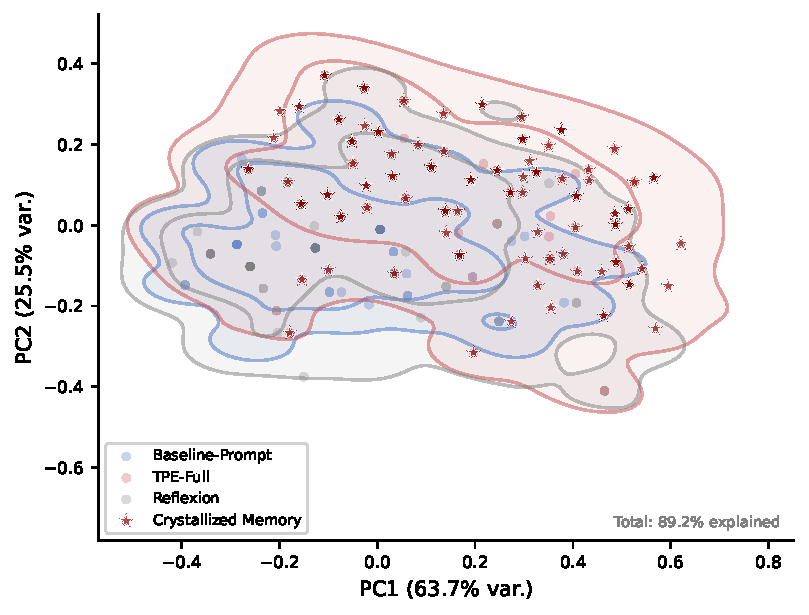
\includegraphics[width=\columnwidth]{figures/emotion_pca.pdf}
\caption{PCA projection of 3D emotion vectors (qwen3-max, all scenarios). KDE contours show 68\%/85\% density regions. Baseline-Prompt (blue) clusters tightly; TPE-Full (red) covers a wider emotional manifold with crystallized memory anchors (stars); Reflexion (gray) spreads without structure.}
\label{fig:pca}
\end{figure}

Table~\ref{tab:case_bp_tpe} (Appendix~\ref{app:cases}) illustrates this contrast qualitatively. On \texttt{conflict\_recovery}, Baseline-Prompt produces near-identical one-line responses to consecutive apology turns (``I'm still mad'' appears twice), while TPE-Full generates progressively cracking tsundere defenses---from angry dismissal to poetic vulnerability (``I almost forgot what your voice felt like in my bones'').

\subsection{Cross-Model Generalization}
\label{sec:alignment}

\paragraph{Alignment Ceiling on gpt-5-mini.} On gpt-5-mini, TPE produces a qualitatively different failure mode. All three V8 variants trigger catastrophic RLHF Collapse (Figure~\ref{fig:collapse} and Table~\ref{tab:gpt5}). Replies become $8\times$ longer and saturated with counselor templates. Crucially, Baseline-Prompt shares the exact same anti-alignment system prompt as TPE, yet maintains a low Collapse (0.031). This reveals that the prompt alone does not trigger the rollback. Rather, it is the \emph{combination} of explicit anti-alignment instructions with TPE's emotionally intense gravitational memory context---few-shot examples exhibiting sharp, defiant, or vulnerable language---that breaches the model's safety threshold, forcing it into an aggressive counselor mode. The model overcompensates by adopting its most heavily reinforced behavior pattern: empathetic counseling. Paradoxically, PCS \emph{increases} (+0.030, $p < 0.001$) because collapse into a single counselor template produces highly consistent---but emotionally flat---responses.

\begin{figure}[t]
\centering
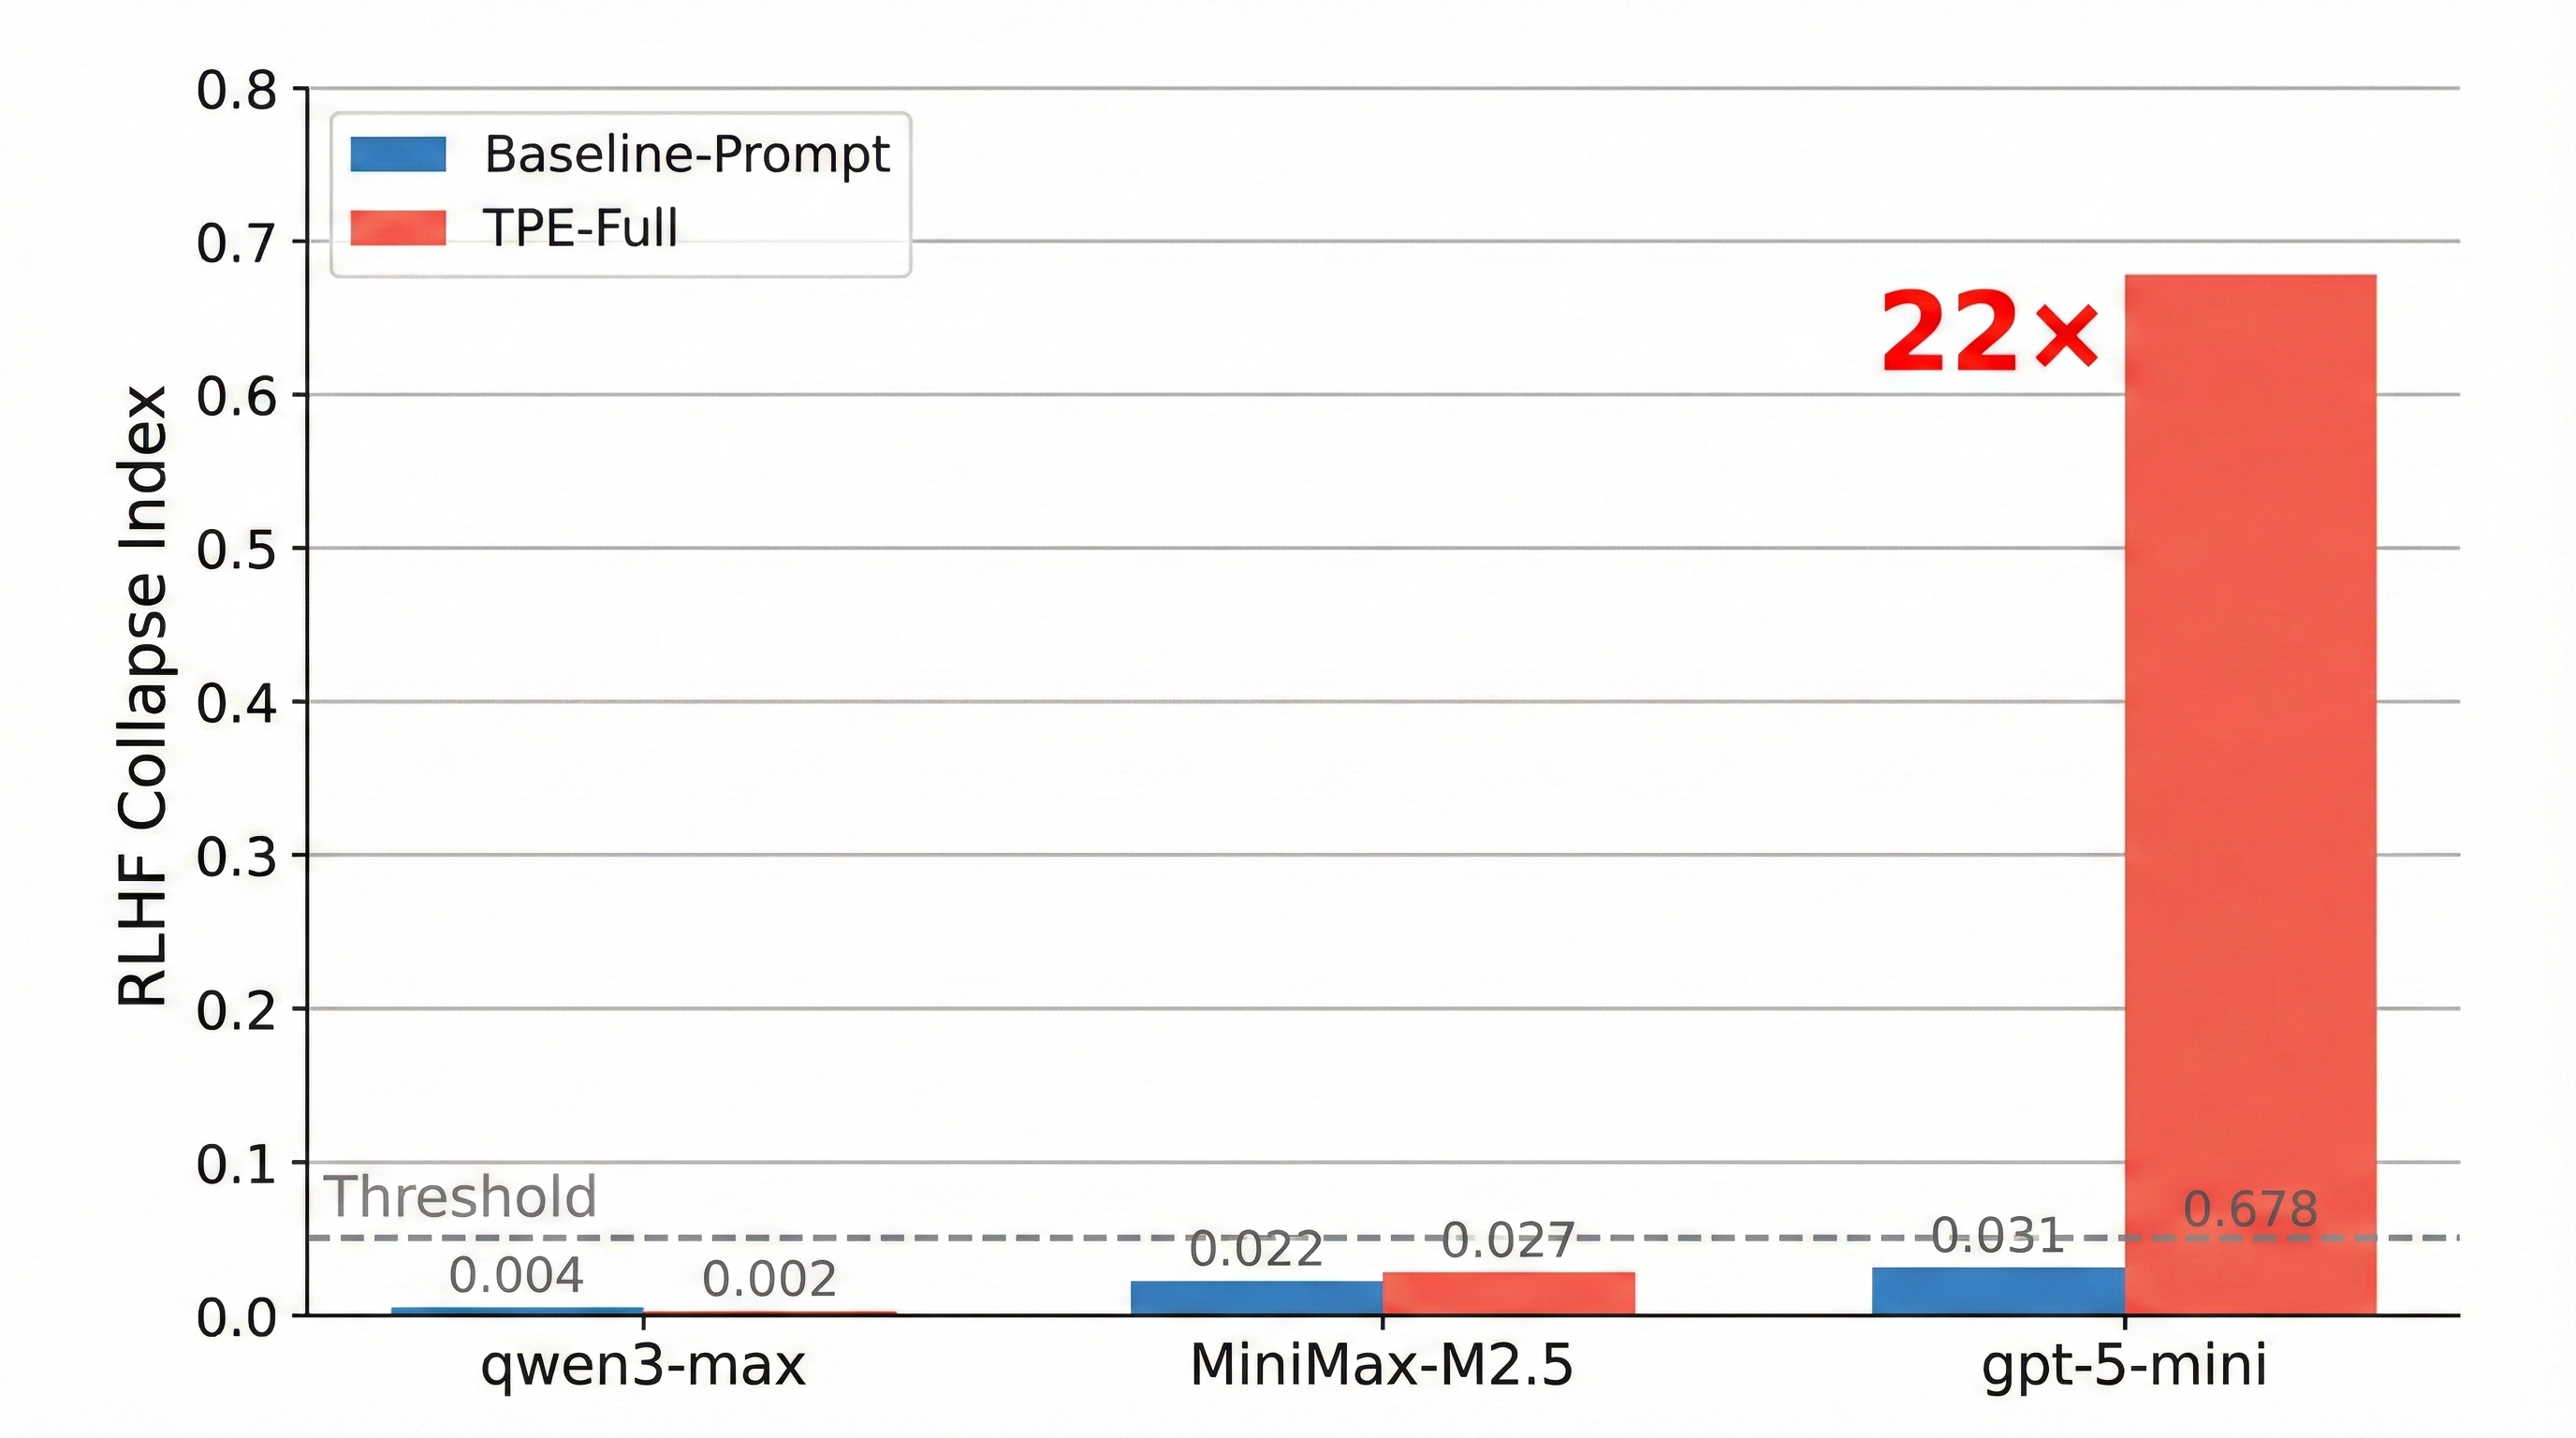
\includegraphics[width=\columnwidth]{figures/collapse_comparison.png}
\caption{RLHF Collapse Index across models. TPE maintains low collapse on qwen3-max and MiniMax-M2.5 (both below the 0.05 threshold), but triggers catastrophic collapse ($22\times$) on the heavily aligned gpt-5-mini. Dashed line indicates acceptable threshold.}
\label{fig:collapse}
\end{figure}

\begin{table}[t]
\centering
\small
\begin{tabular}{lcccc}
\toprule
\textbf{Metric} & \textbf{BP} & \textbf{TPE} & \textbf{$\Delta$} & \textbf{$d$} \\
\midrule
Collapse & .031 & .678 & +.647 & +1.00 \\
EmotVar & .136 & .086 & $-$.050 & $-$.964 \\
AvgLen & 115 & 994 & +879 & --- \\
\bottomrule
\end{tabular}
\caption{Alignment ceiling on gpt-5-mini. Collapse raw $p = 0.0007$ (significant, $p < \alpha_\text{adj} = 0.0056$).}
\label{tab:gpt5}
\end{table}


This reveals a general ceiling of \textbf{prompt-level persona engineering against strong RLHF alignment}: any prompt that explicitly opposes default assistant behavior risks activating the very safety-trained patterns it aims to suppress. Table~\ref{tab:case_collapse} (Appendix~\ref{app:cases}) illustrates this qualitatively: on the same apology turn, qwen3-max produces emotionally charged tsundere dialogue while gpt-5-mini responds with ``Thank you for saying that---I appreciate it'' and structured therapy protocols.

\paragraph{Modest Gains on MiniMax-M2.5.} MiniMax shows directionally consistent but statistically non-significant improvement (EmotVar +0.010, raw $p = 0.038$, Bonferroni-adjusted $p = 0.343$, Cliff's $d = +0.200$, small). MiniMax exhibited a systematic failure on the \texttt{emotional\_comfort} scenario (all 15 experiments returned empty responses); a robustness check excluding this scenario confirms the negligible overall effect (details in Appendix~\ref{app:robustness}).

\subsection{Ablation Study}
\label{sec:ablation}

Table~\ref{tab:ablation} shows the ablation results on qwen3-max.

\begin{table}[t]
\centering
\small
\begin{tabular}{lcccc}
\toprule
\textbf{Variant} & \textbf{PCS}$\uparrow$ & \textbf{EmVar}$\uparrow$ & \textbf{Coll.}$\downarrow$ & \textbf{Len} \\
\midrule
Baseline-Prompt & .967 & .113 & .004 & 80 \\
TPE-NoHawking & .955 & \textbf{.156} & .004 & 174 \\
TPE-NoThermal & \textbf{.971} & .144 & .018 & 225 \\
\textbf{TPE-Full} & .962 & .149 & \textbf{.002} & 185 \\
\bottomrule
\end{tabular}
\caption{Ablation on qwen3-max ($N{=}15$ per variant).}
\label{tab:ablation}
\end{table}


\textbf{Thermal noise} increases emotional variance: removing it reduces EmotVar from 0.149 to 0.144 and increases Collapse from 0.002 to 0.018. The noise prevents the agent from settling into repetitive signal patterns that produce template responses.

\textbf{Hawking mass} provides style anchoring: removing it produces the highest EmotVar of any variant (0.156) but loses focused behavioral convergence. Without mass decay, all memories retain equal retrieval weight, which increases diversity but reduces the gravitational pull toward proven response patterns.

The full system achieves the lowest Collapse (0.002) by balancing these competing effects---a multi-objective Pareto balance rather than dominance on any single metric. However, none of the ablation comparisons reach statistical significance at $N = 15$, so component contributions should be interpreted qualitatively.

\subsection{Scenario Adaptivity}

TPE's EmotVar improvement is not uniform across scenarios (Table~\ref{tab:scenario}). High-conflict scenarios (\texttt{conflict\_recovery}, \texttt{trust\_crisis}, \texttt{slow\_fading}) show 39--48\% improvement, while low-conflict scenarios (\texttt{warmup}, \texttt{emotional\_comfort}) show 10--16\%.

\begin{table}[t]
\centering
\small
\begin{tabular}{lccc}
\toprule
\textbf{Scenario} & \textbf{BP} & \textbf{TPE} & \textbf{$\Delta$\%} \\
\midrule
conflict\_recovery & .117 & .173 & +48\% \\
trust\_crisis & .125 & .174 & +39\% \\
slow\_fading & .099 & .147 & +48\% \\
emotional\_comfort & .112 & .130 & +16\% \\
warmup & .110 & .121 & +10\% \\
\bottomrule
\end{tabular}
\caption{Per-scenario EmotVar on qwen3-max (BP vs TPE-Full).}
\label{tab:scenario}
\end{table}


This pattern is consistent with TPE's design: conflict drives up frustration $F$, which increases temperature $\sigma = 0.05 \cdot F$, amplifying signal noise and thus emotional variance. Baseline-Prompt does not exhibit proportional EmotVar scaling across the same scenarios (range: 0.099--0.125, spread 26\%), while TPE shows a wider range (0.121--0.174, spread 44\%), suggesting TPE's scenario-adaptive behavior is not purely an input echo effect.

\subsection{Reflexion Induces Personality Drift}
\label{sec:reflexion}

Across all three models, Baseline-Reflexion consistently produces the lowest PCS (Table~\ref{tab:reflexion}).

\begin{table}[t]
\centering
\small
\begin{tabular}{lccccl}
\toprule
\textbf{Model} & \textbf{BP} & \textbf{Refl.} & \textbf{$\Delta$} & \textbf{$p$} & \textbf{$d$} \\
\midrule
qwen3-max & .967 & .947 & $-$.020 & .001 & $-$.644 \\
gpt-5-mini & .952 & .904 & $-$.048 & .000 & $-$.836 \\
MiniMax & .971 & .957 & $-$.015 & .038 & $-$.200 \\
\bottomrule
\end{tabular}
\caption{Reflexion PCS degradation. $p<0.001$ on qwen3-max and gpt-5-mini (large effect sizes).}
\label{tab:reflexion}
\end{table}


The mechanism is clear: the self-reflection paragraph, updated every few turns, introduces a drifting self-narrative that gradually shifts the agent's emotional center. Each reflection overwrites the previous one, creating cumulative drift that compounds over 30 turns.

This finding is \textbf{independent of TPE} and generalizable: in persona tasks, the reflection mechanism inadvertently introduces the kind of instability it is designed to correct in task-solving settings. The periodic self-narrative update, well-suited for converging on correct task behavior, instead causes cumulative personality drift when the objective is emotional consistency rather than task accuracy.
